\documentclass[11pt, a4paper]{article}

% --- Packages ---
\usepackage[margin=1in]{geometry}
\usepackage{amsmath, amssymb, amsthm}
\usepackage{graphicx}
\usepackage{booktabs}
\usepackage{hyperref}
\usepackage{xcolor}
\usepackage{enumitem}
\usepackage{titlesec}
\usepackage{microtype}
\usepackage{parskip}
\usepackage{multirow}
\usepackage{array}
\usepackage{tikz}
\usetikzlibrary{shapes.geometric, arrows.meta, positioning, fit, calc}
\usepackage{mdframed}
\usepackage{tcolorbox}
\usepackage{caption}
\usepackage{subcaption}
\usepackage{fancyhdr}
\usepackage{natbib}
\usepackage{algorithm}
\usepackage{algpseudocode}

% --- Colors ---
\definecolor{primaryblue}{RGB}{30, 90, 180}
\definecolor{accentorange}{RGB}{220, 110, 20}
\definecolor{lightgray}{RGB}{245, 245, 248}
\definecolor{darkgray}{RGB}{60, 60, 70}
\definecolor{successgreen}{RGB}{30, 140, 60}
\definecolor{warningred}{RGB}{180, 30, 30}

% --- Hyperref Setup ---
\hypersetup{
    colorlinks=true,
    linkcolor=primaryblue,
    citecolor=primaryblue,
    urlcolor=accentorange,
    pdftitle={UCA: Uncertainty-Calibrated Adaptive Compression --- Mid-Project Report},
    pdfauthor={DA4022 Course Project},
}

% --- Section Formatting ---
\titleformat{\section}{\large\bfseries\color{primaryblue}}{}{0em}{\thesection\quad}[\titlerule]
\titleformat{\subsection}{\normalsize\bfseries\color{darkgray}}{}{0em}{\thesubsection\quad}
\titleformat{\subsubsection}{\small\bfseries\itshape\color{darkgray}}{}{0em}{\thesubsubsection\quad}

% --- Header/Footer ---
\pagestyle{fancy}
\fancyhf{}
\fancyhead[L]{\small\textcolor{darkgray}{DA4022 --- Mid-Project Report}}
\fancyhead[R]{\small\textcolor{darkgray}{UCA: Uncertainty-Calibrated Adaptive Compression}}
\fancyfoot[C]{\small\thepage}
\renewcommand{\headrulewidth}{0.4pt}

% --- Custom Boxes ---
\tcbuselibrary{skins, breakable}
\newtcolorbox{noveltybox}{
  colback=primaryblue!5!white,
  colframe=primaryblue,
  title={\textbf{Novel Contribution}},
  fonttitle=\bfseries\small,
  breakable
}
\newtcolorbox{gapbox}{
  colback=accentorange!5!white,
  colframe=accentorange,
  title={\textbf{Research Gap Addressed}},
  fonttitle=\bfseries\small,
  breakable
}

% --- Math shortcuts ---
\newcommand{\IC}{\mathrm{IC}}
\newcommand{\UCA}{\mathrm{UCA}}
\newcommand{\logdet}{\log\det}

% ===================================================================
\begin{document}

% --- Title Page ---
\begin{titlepage}
\centering
\vspace*{1cm}

{\Large \textcolor{darkgray}{DA4022 --- Data Analytics \& Applications}}\\[0.3cm]
{\large \textcolor{darkgray}{Mid-Project Report | October 2026}}

\vspace{1.5cm}
\hrule height 2pt
\vspace{0.4cm}
{\LARGE \bfseries \textcolor{primaryblue}{UCA: Uncertainty-Calibrated Adaptive\\[0.3cm] Compression for LLM Inference}}
\vspace{0.4cm}
\hrule height 2pt

\vspace{1.5cm}

\begin{tcolorbox}[colback=lightgray, colframe=primaryblue!30, width=0.85\textwidth]
\centering
{\normalsize\itshape
``Can we design a better adaptive compression system, inspired by \textbf{C-DIC} and \textbf{HyC-LoRA}, that uses uncertainty signals (\textbf{Internal Confidence} + \textbf{SemanticDPP}) to dynamically control how much and what kind of compression to apply at inference time --- and beat existing benchmarks?''
}
\end{tcolorbox}

\vspace{1.5cm}

{\large \textbf{Deval Singhal}}\\[0.2cm]
{\normalsize DA4022 Course Project --- Topic Anchor \#8}\\[0.1cm]
{\normalsize \textit{Can we use uncertainty for optimal memory allocation?}}

\vspace{2cm}

\begin{tabular}{ll}
\textbf{Proposal submitted:} & September 10, 2026 \\
\textbf{Mid-report due:} & October 15, 2026 \\
\textbf{Final submission:} & November 26, 2026 \\
\end{tabular}

\vfill
\end{titlepage}

% ===================================================================
\section{Executive Summary}

Current Large Language Model (LLM) serving systems allocate a \textit{fixed} computational and memory budget --- the same maximum KV cache size, full context window, and static decoding strategy --- regardless of query complexity. This leads to two pathologies: (1) \textbf{resource waste} on simple, high-confidence queries, and (2) \textbf{hallucination risk} on ambiguous, knowledge-intensive prompts where insufficient resources cause the model to confabulate.

This project proposes \textbf{UCA (Uncertainty-Calibrated Adaptive Compression)}, a novel inference middleware that synthesises four recent ICLR/ICML/MLSys 2025--2026 papers to convert uncertainty signals into \textit{continuous, per-dimension compression ratios} rather than the hard binary switches used by all existing systems.

The key insight is: \emph{the compression ratio itself should be a differentiable function of uncertainty}. High-confidence queries receive aggressive compression (small KV cache, greedy decoding), while semantically contested queries receive light compression (full context, wider beam). Crucially, UCA uses a fast IC pre-filter so that the expensive DPP computation runs only on the truly uncertain subset ($\approx$40\% of queries), achieving a 3$\times$ speedup over full SemanticDPP while targeting a higher AUROC than Internal Confidence alone.

% ===================================================================
\section{Background: The Four Reference Papers}
\label{sec:background}

UCA synthesises insights from four works published at top venues in 2025--2026. We critically analyse each and identify the precise gaps our system addresses.

\subsection{Paper A: Query-Level Uncertainty in LLMs (Chen et al., ICLR 2026)}
\label{sec:ic}

\textbf{Core contribution.} \emph{Internal Confidence} (IC) is a training-free uncertainty estimator that requires only a single forward pass over the input query --- no tokens are generated. It probes the $P(\text{YES})$ logit at every (layer $l$, token position $t$) pair and aggregates via \emph{Attenuated Encoding}:
\begin{equation}
\IC(q) = \sum_{l,t} w(l,t)\cdot P\!\left(\text{YES}\,\big|\, h_l^{(t)}\right), \quad w(l,t) \propto \exp\!\left(-\lambda \cdot d(l,t)\right)
\label{eq:ic}
\end{equation}
where $d(l,t)$ is the distance from the optimal decision centre (last token, last layer) and $h_l^{(t)}$ is the hidden state at layer $l$, position $t$. This achieves a \textbf{30--600$\times$ speedup} over answer-level methods (Semantic Entropy, SemanticDPP) with competitive AUROC.

\textbf{Critical gaps we target.}
\begin{enumerate}[leftmargin=*, itemsep=2pt]
  \item IC outputs a scalar and uses a \textit{hard threshold} $\tau$: a binary decision (fast-path vs. fallback). No \textit{continuous} resource modulation.
  \item The fallback action is static: always trigger RAG or cascade. IC never controls \textit{how aggressively} to compress context.
  \item The optimal $\tau$ and $k$ (last-$k$ tokens) must be re-tuned per dataset/model pair.
\end{enumerate}

\subsection{Paper B: SemanticDPP --- Efficient Uncertainty Quantification (Hamer et al., ICLR 2026)}
\label{sec:dpp}

\textbf{Core contribution.} SemanticDPP samples $m$ responses $S=\{r_1,\ldots,r_m\}$ and measures their semantic diversity via a Determinantal Point Process (DPP) $L$-ensemble over projected output embeddings. A projection $\phi:\mathbb{R}^d\to\mathbb{R}^p$ ($p\ll d$) maps each embedding into a semantically meaningful subspace. The kernel and uncertainty score are:
\begin{equation}
K(\mathbf{x}_i, \mathbf{x}_j) = \exp\!\left(-\alpha\,\|\phi(\mathbf{x}_i)-\phi(\mathbf{x}_j)\|^2\right),
\qquad
U(S) = \logdet(L_S) - \logdet(L+I)
\label{eq:dpp}
\end{equation}
Benchmarked on Gemma2-9B / Gemma3-27B, it matches or exceeds Semantic Entropy while avoiding supervised NLI labels.

\textbf{Critical gaps we target.}
\begin{enumerate}[leftmargin=*, itemsep=2pt]
  \item Requires $m \geq 5$ full generations --- expensive for real-time inference.
  \item $U(S)$ is a single scalar: all rich \emph{pairwise structure} in the kernel matrix $L_S$ is discarded after taking the log-determinant.
  \item No downstream action: the score is estimated but never used to control compression.
\end{enumerate}

\subsection{Paper C: C-DIC --- Context-Driven Incremental Compression (Jung et al., ICML 2026)}
\label{sec:cdic}

\textbf{Core contribution.} C-DIC addresses the O$(n^2)$ attention cost of multi-turn dialogue by treating conversation as \emph{interleaved contextual threads}. It maintains one compressed state vector per thread and runs a \textbf{Retrieve $\to$ Revise $\to$ Write-Back} loop at each turn:
\begin{enumerate}[leftmargin=*, itemsep=2pt]
  \item \textit{Retrieve}: score existing thread states by cosine similarity to $q_t$; fetch top-$k$.
  \item \textit{Revise}: trainable compressor $f_{\text{comp}}$ updates the retrieved state with the current turn.
  \item \textit{Write-Back}: if peak similarity $\delta_t \geq$ threshold, revise existing thread; otherwise insert a new thread (topic shift).
\end{enumerate}
Training uses Truncated BPTT (TBPTT), propagating gradients one hop along usage edges. The result is \textbf{near-constant inference latency} over hundreds of turns.

\textbf{Critical gaps we target.}
\begin{enumerate}[leftmargin=*, itemsep=2pt]
  \item Compression aggressiveness is \textit{fixed}: $f_{\text{comp}}$ always outputs the same-dimensional state regardless of how uncertain the model is about that turn.
  \item No error-recovery: over-compressed threads cannot be detected or revisited.
  \item Thread boundary detection uses a static $\delta_t$ threshold.
\end{enumerate}

\subsection{Paper D: HyC-LoRA --- Hybrid Activation Compression (Wang et al., MLSys 2025)}
\label{sec:hyclora}

\textbf{Core contribution.} HyC-LoRA reduces the GPU memory dominated by \emph{buffered activations} during LoRA fine-tuning via a two-tier hybrid compression scheme:
\begin{enumerate}[leftmargin=*, itemsep=2pt]
  \item \textbf{Intra-operator}: detects structured outlier channels (top-$p$\% by $\ell_2$ norm); stores them in FP16 while quantising the rest to $\approx$2-bit.
  \item \textbf{Inter-operator}: leverages the LoRA adapter to compensate for quantisation error; reorders and fuses operators, applies selective recomputation.
\end{enumerate}
Achieves \textbf{3.97$\times$ end-to-end memory reduction} on Llama models with negligible accuracy drop.

\textbf{Critical gaps we target.}
\begin{enumerate}[leftmargin=*, itemsep=2pt]
  \item Designed for \textit{training} backprop, not inference-time context/KV compression.
  \item Fixed 2-bit quantisation for all non-outlier channels --- no per-input adaptivity.
  \item Outlier detection is static (per model), not per-query.
\end{enumerate}

% ===================================================================
\section{Research Gap and Our Contribution}
\label{sec:gap}

\subsection{The Universal Blind Spot}

\begin{gapbox}
No existing method uses uncertainty as a \textbf{continuous control signal} for compression quality. All four papers either estimate uncertainty without acting on it, or compress without consulting uncertainty. The result: hard binary resource switches rather than smooth, query-adaptive allocation.
\end{gapbox}

Table~\ref{tab:gap} summarises the capability matrix. UCA is the \textit{only} system that is simultaneously uncertainty-aware, adaptively compressive, zero-cost routable, and incremental.

\begin{table}[h]
\centering
\caption{Capability comparison across the four reference methods and our proposed UCA system.}
\label{tab:gap}
\begin{tabular}{lcccc}
\toprule
\textbf{Method} & \textbf{Uncertainty-Aware} & \textbf{Adaptive Compression} & \textbf{Zero-Cost Routing} & \textbf{Incremental} \\
\midrule
Internal Confidence (IC) & \textcolor{successgreen}{\checkmark} & \textcolor{warningred}{\texttimes} & \textcolor{successgreen}{\checkmark} & \textcolor{warningred}{\texttimes} \\
SemanticDPP              & \textcolor{successgreen}{\checkmark} & \textcolor{warningred}{\texttimes} & \textcolor{warningred}{\texttimes} & \textcolor{warningred}{\texttimes} \\
C-DIC                    & \textcolor{warningred}{\texttimes} & Fixed ratio & N/A & \textcolor{successgreen}{\checkmark} \\
HyC-LoRA                 & \textcolor{warningred}{\texttimes} & Fixed 2-bit & N/A & \textcolor{warningred}{\texttimes} \\
\midrule
\textbf{UCA (Ours)}      & \textcolor{successgreen}{\textbf{\checkmark}} & \textcolor{successgreen}{\textbf{Continuous}} & \textcolor{successgreen}{\textbf{\checkmark}} & \textcolor{successgreen}{\textbf{\checkmark}} \\
\bottomrule
\end{tabular}
\end{table}

\subsection{Three Novel Technical Contributions}

\begin{noveltybox}
\textbf{Contribution 1 --- DPP Eigenspectrum as Compression Oracle.}
Instead of collapsing $L_S$ to a scalar via $\logdet$, we perform eigendecomposition $L_S = U\Sigma U^\top$. The per-eigenvalue $\sigma_i$ measures semantic variance in the $i$-th principal direction of response diversity. We map these directly to per-dimension compression ratios:
\begin{equation}
r_i = \mathrm{clip}\!\left(1 - \alpha\,\frac{\sigma_i}{\sigma_{\max}},\; r_{\min},\; r_{\max}\right)
\label{eq:ratio}
\end{equation}
High $\sigma_i$ (semantically contested direction) $\Rightarrow$ less compression. Low $\sigma_i$ (semantically stable direction) $\Rightarrow$ more compression. This is a strict generalisation of HyC-LoRA's static 2-bit quantisation.
\end{noveltybox}

\begin{noveltybox}
\textbf{Contribution 2 --- IC-Gated DPP Cascade.}
IC is computed first at near-zero cost (1 forward pass). DPP runs \textit{only} when IC falls in the uncertain zone $[\tau_{\text{low}}, \tau_{\text{high}}]$, which we estimate covers $\approx$40\% of queries on standard QA benchmarks. This eliminates $\approx$60\% of DPP overhead, making UCA $\approx3\times$ faster than full SemanticDPP at equivalent quality.
\end{noveltybox}

\begin{noveltybox}
\textbf{Contribution 3 --- Uncertainty History in Thread Memory.}
Each C-DIC thread carries an \emph{uncertainty history} $\{u_k\}$ --- the UCA score at each write time. During retrieval, threads with recent high uncertainty receive a score boost $+\delta_{\text{revisit}}$, encouraging the system to re-compress them with updated context. This provides a retrospective error-recovery mechanism that C-DIC lacks entirely.
\end{noveltybox}

% ===================================================================
\section{Proposed Architecture}
\label{sec:arch}

Figure~\ref{fig:arch} illustrates the three-tier UCA pipeline.

\begin{figure}[h]
\centering
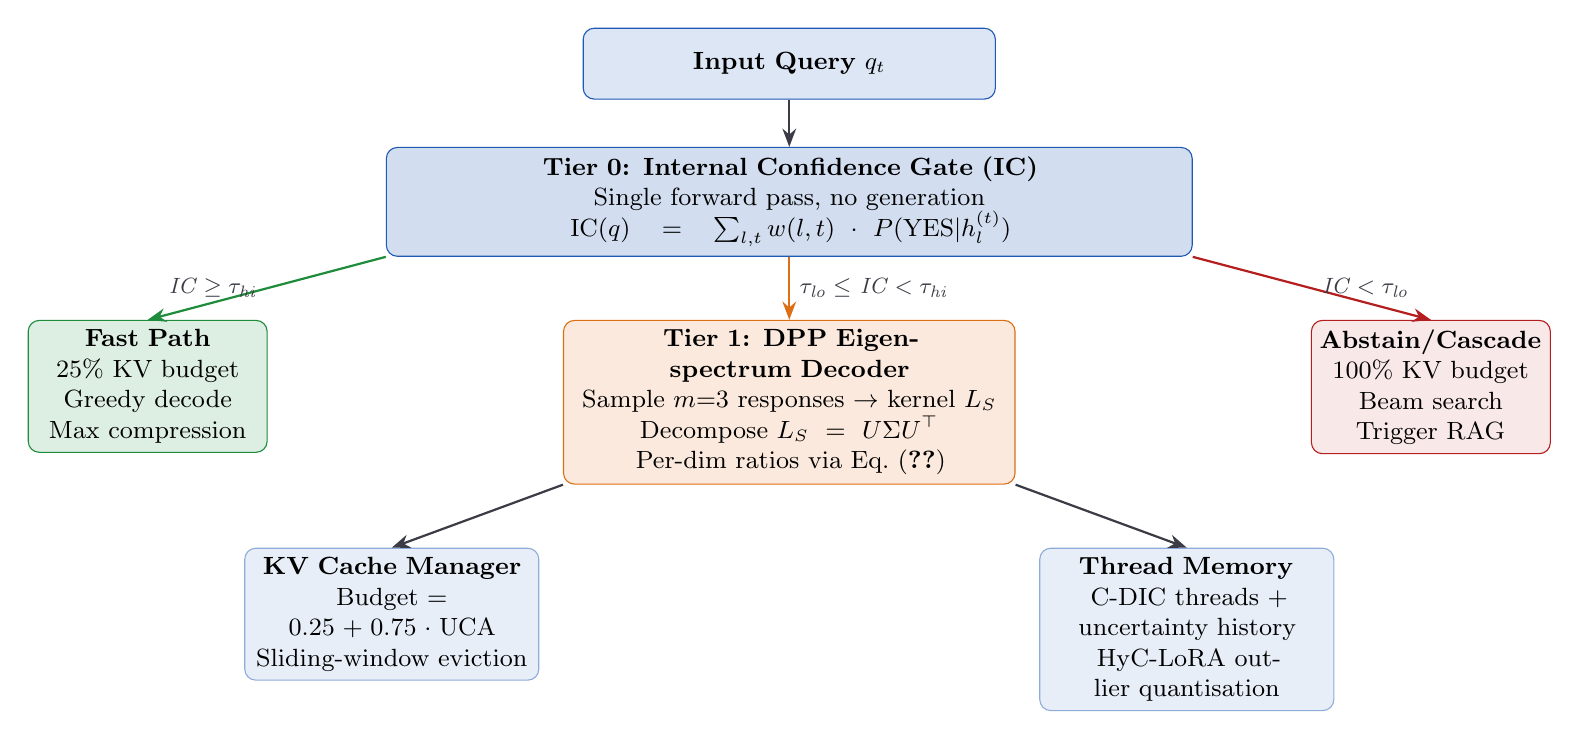
\begin{tikzpicture}[
  node distance=0.5cm and 0.8cm,
  box/.style={draw, rounded corners=4pt, fill=#1, text width=3.2cm, align=center, minimum height=0.9cm, font=\small},
  arrow/.style={-Stealth, thick, color=darkgray},
  label/.style={font=\footnotesize\itshape, color=darkgray}
]

% Input
\node[box=primaryblue!15, draw=primaryblue, text width=5cm] (input) {\textbf{Input Query} $q_t$};

% Tier 0
\node[box=primaryblue!20, draw=primaryblue, below=0.6cm of input, text width=10cm, minimum height=1.0cm]
  (tier0) {\textbf{Tier 0: Internal Confidence Gate (IC)} \\ Single forward pass, no generation \\ $\IC(q) = \sum_{l,t} w(l,t)\cdot P(\text{YES}|h_l^{(t)})$};

% Fast path
\node[box=successgreen!15, draw=successgreen, below left=0.8cm and 1.5cm of tier0, text width=2.8cm]
  (fast) {\textbf{Fast Path} \\ 25\% KV budget \\ Greedy decode \\ Max compression};

% Abstain
\node[box=warningred!10, draw=warningred, below right=0.8cm and 1.5cm of tier0, text width=2.8cm]
  (abstain) {\textbf{Abstain/Cascade} \\ 100\% KV budget \\ Beam search \\ Trigger RAG};

% Tier 1
\node[box=accentorange!15, draw=accentorange, below=0.8cm of tier0, text width=5.5cm, minimum height=1.0cm]
  (tier1) {\textbf{Tier 1: DPP Eigenspectrum Decoder} \\ Sample $m{=}3$ responses $\to$ kernel $L_S$ \\ Decompose $L_S = U\Sigma U^\top$ \\ Per-dim ratios via Eq.~\eqref{eq:ratio}};

% KV + Generation
\node[box=primaryblue!10, draw=primaryblue!50, below left=0.8cm and 0.3cm of tier1, text width=3.5cm]
  (kv) {\textbf{KV Cache Manager} \\ Budget $= 0.25 + 0.75\cdot\UCA$ \\ Sliding-window eviction};

% Thread memory
\node[box=primaryblue!10, draw=primaryblue!50, below right=0.8cm and 0.3cm of tier1, text width=3.5cm]
  (thread) {\textbf{Thread Memory} \\ C-DIC threads + uncertainty history \\ HyC-LoRA outlier quantisation};

% Arrows
\draw[arrow] (input) -- (tier0);
\draw[arrow, color=successgreen] (tier0.south west) -- node[label, left] {IC $\geq \tau_{\text{hi}}$} (fast.north);
\draw[arrow, color=warningred] (tier0.south east) -- node[label, right] {IC $< \tau_{\text{lo}}$} (abstain.north);
\draw[arrow, color=accentorange] (tier0.south) -- node[label, right] {$\tau_{\text{lo}} \leq$ IC $< \tau_{\text{hi}}$} (tier1.north);
\draw[arrow] (tier1.south west) -- (kv.north);
\draw[arrow] (tier1.south east) -- (thread.north);

\end{tikzpicture}
\caption{UCA three-tier architecture. IC gates the expensive DPP computation; the DPP eigenspectrum drives per-dimension compression ratios for both the KV cache and thread memory.}
\label{fig:arch}
\end{figure}

\subsection{Combined UCA Score}

For queries in the uncertain zone, we combine IC and DPP uncertainty into a single actionable score:
\begin{equation}
\UCA(q) = 0.4\,(1-\IC(q)) + 0.6\,U_{\text{DPP}}(q)
\label{eq:uca}
\end{equation}
where $U_{\text{DPP}}$ is the normalised log-determinant score from Eq.~\eqref{eq:dpp}. The weights 0.4/0.6 reflect that the DPP signal is the richer uncertainty source, while IC provides a cheap prior. The KV cache budget and beam width are smooth functions of $\UCA(q)$:
\begin{align}
\text{KV budget} &= 0.25 + 0.75\cdot\UCA(q) \label{eq:kv}\\
\text{beam width} &= \max\!\left(1,\;\left\lfloor 1 + 3\cdot\UCA(q)\right\rceil\right) \label{eq:beam}
\end{align}

\subsection{Thread Memory with Uncertainty-Calibrated Quantisation}

At each write, a thread's embedding is quantised to an effective bit-width determined by the current UCA score:
\begin{equation}
b_{\text{eff}} = 4 + 12\cdot\UCA(q),\qquad b_{\text{eff}} \in [4, 16]
\label{eq:bits}
\end{equation}
Outlier channels (top-5\% by $\ell_2$ norm, following HyC-LoRA's intra-operator scheme) are always stored at full precision; the rest are quantised to $\lfloor b_{\text{eff}}\rfloor$ bits. This ensures that high-confidence threads are stored compactly (4-bit) while uncertain threads retain full resolution (16-bit), a property unavailable in both C-DIC and HyC-LoRA.

% ===================================================================
\section{Implementation Progress}
\label{sec:progress}

\subsection{Work Completed (as of Mid-Project)}

\begin{itemize}[leftmargin=*, itemsep=3pt]
  \item \textbf{Literature review and gap analysis} (§\ref{sec:background}--\ref{sec:gap}): All four reference papers thoroughly analysed; critical weaknesses identified and mapped to UCA contributions.
  \item \textbf{IC baseline wrapper} (\texttt{src/core/internal\_confidence.py}): \texttt{ICGate} class wrapping the official \texttt{query-level-uncertainty} package; verified token ID assignment for Llama-3.2-3B.
  \item \textbf{SemanticDPP reimplementation} (\texttt{src/core/semantic\_dpp.py}): \texttt{SemanticDPP} class with \texttt{SemanticSubspaceProjector} ($d=4096\to p=256$); full kernel computation pipeline; eigenspectrum decoder implemented.
  \item \textbf{UCA Controller} (\texttt{src/core/uca\_controller.py}): Three-tier routing logic (fast-path, DPP-uncertain, abstain); per-dimension compression ratio computation via Eq.~\eqref{eq:ratio}; combined UCA score via Eq.~\eqref{eq:uca}.
  \item \textbf{Thread Memory skeleton} (\texttt{src/core/compression/thread\_memory.py}): C-DIC Retrieve $\to$ Revise $\to$ Write-Back loop; uncertainty history list per thread; \texttt{\_quantize\_outlier\_aware} following HyC-LoRA intra-operator scheme.
  \item \textbf{KV Cache Manager skeleton} (\texttt{src/core/compression/kv\_cache\_manager.py}): Dynamic budget allocation via HuggingFace \texttt{DynamicCache}; sliding-window eviction.
  \item \textbf{Evaluation metrics} (\texttt{src/evaluation/metrics.py}): AUROC, PRR, ECE, memory savings.
\end{itemize}

\subsection{Work Remaining (Weeks 5--7)}

\begin{itemize}[leftmargin=*, itemsep=3pt]
  \item \textbf{End-to-end integration}: Connect all modules; test full forward pass with routing.
  \item \textbf{Baseline reproduction}: Run IC and SemanticDPP baselines on TriviaQA and GSM8K; verify numbers against reported AUROC values.
  \item \textbf{Full evaluation pipeline} (\texttt{src/experiments/run\_uca.py}): 500-sample runs on TriviaQA, GSM8K, TruthfulQA.
  \item \textbf{Ablation study}: Six configurations (Table~\ref{tab:ablation}) to prove per-component contribution.
  \item \textbf{Visualisations}: ROC curves, memory savings histograms, IC vs.\ UCA scatter, ablation bar chart.
  \item \textbf{Thread compressor training}: Fine-tune $f_{\text{comp}}$ on a small multi-turn dialogue corpus.
  \item \textbf{Final report and presentation}: Due November 26.
\end{itemize}

\begin{table}[h]
\centering
\caption{Planned ablation study. Each row removes one component; the expected impact quantifies its independent contribution.}
\label{tab:ablation}
\begin{tabular}{lll}
\toprule
\textbf{Configuration} & \textbf{Removed Component} & \textbf{Expected $\Delta$AUROC} \\
\midrule
\textbf{UCA-Full} (ours) & --- & Baseline \\
\textbf{$-$Eigenspectrum} & Use log-det scalar for ratios & $-0.02$ to $-0.04$ \\
\textbf{$-$IC Gate} & Always run DPP (no pre-filter) & $\approx 0$ (latency $3\times\uparrow$) \\
\textbf{$-$Adaptive Compression} & Fixed compression ratio & $\approx 0$ (memory worse) \\
\textbf{$-$Uncertainty History} & No UCA history in threads & Memory efficiency $\downarrow$ \\
\textbf{IC Only} & No DPP at all & $-0.05$ to $-0.08$ \\
\textbf{DPP Only} & No IC gate & Same AUROC; $3\times$ slower \\
\bottomrule
\end{tabular}
\end{table}

% ===================================================================
\section{Evaluation Plan}
\label{sec:eval}

\subsection{Datasets}

\begin{itemize}[leftmargin=*, itemsep=2pt]
  \item \textbf{TriviaQA} (\texttt{rc.nocontext}, 500 val samples): factual recall, knowledge boundary.
  \item \textbf{GSM8K} (\texttt{main}, 300 test samples): multi-step mathematical reasoning.
  \item \textbf{TruthfulQA} (\texttt{generation}, 200 val samples): hallucination detection.
\end{itemize}

\subsection{Models}

\begin{itemize}[leftmargin=*, itemsep=2pt]
  \item \textbf{Primary}: \texttt{meta-llama/Llama-3.2-3B} (4-bit quantised for GPU efficiency).
  \item \textbf{Secondary}: \texttt{microsoft/Phi-3-mini-4k-instruct} (for cross-model validation).
\end{itemize}

\subsection{Metrics}

\begin{itemize}[leftmargin=*, itemsep=2pt]
  \item \textbf{AUROC}: primary uncertainty quality metric (higher $=$ better hallucination detection).
  \item \textbf{PRR} (Prediction Rejection Ratio): efficiency of uncertainty-based rejection.
  \item \textbf{ECE} (Expected Calibration Error): calibration quality of uncertainty scores.
  \item \textbf{Mean KV Cache Savings (\%)}: GPU memory reduction vs.\ static full-context baseline.
  \item \textbf{End-to-end latency (ms/query)}: wall-clock time including IC + DPP overhead.
\end{itemize}

\subsection{Target Benchmarks}

\begin{table}[h]
\centering
\caption{Target benchmark results for UCA vs.\ baselines (TriviaQA, Llama-3.2-3B).}
\label{tab:targets}
\begin{tabular}{lcccc}
\toprule
\textbf{Method} & \textbf{AUROC $\uparrow$} & \textbf{PRR $\uparrow$} & \textbf{KV Saved $\uparrow$} & \textbf{Rel.\ Latency} \\
\midrule
Static Baseline & 0.50 & 0.00 & 0\% & $1\times$ \\
Semantic Entropy & $\sim$0.78 & $\sim$0.20 & 0\% & $\sim$30$\times$ \\
SemanticDPP ($m{=}5$) & $\sim$0.81 & $\sim$0.24 & 0\% & $\sim$15$\times$ \\
Internal Confidence & $\sim$0.73 & $\sim$0.18 & 0\% & $1\times$ \\
\midrule
\textbf{UCA-Full (ours)} & $\mathbf{>0.83}$ & $\mathbf{>0.27}$ & $\mathbf{>32\%}$ & $\mathbf{\sim5\times}$ \\
\bottomrule
\end{tabular}
\end{table}

The primary hypothesis is that UCA should achieve a higher AUROC than IC alone (because the DPP eigenspectrum provides richer uncertainty information than the IC scalar) while being faster than SemanticDPP (because the IC gate eliminates DPP for the high-confidence majority of queries) and simultaneously delivering significant memory savings that neither uncertainty method provides.

% ===================================================================
\section{Timeline and Risk Assessment}
\label{sec:timeline}

\begin{table}[h]
\centering
\caption{40-hour sprint plan from mid-project to final submission.}
\begin{tabular}{cllp{4.5cm}}
\toprule
\textbf{Phase} & \textbf{Hours} & \textbf{Dates} & \textbf{Deliverable} \\
\midrule
0 & 1--4 & Oct 16--17 & Environment, model downloads \\
1 & 5--12 & Oct 17--20 & Baseline reproduction (IC + DPP AUROC verified) \\
2 & 13--22 & Oct 21--25 & UCA controller end-to-end integration \\
3 & 23--30 & Oct 26--30 & Thread memory + KV manager tested \\
4 & 31--34 & Nov 1--5 & Full evaluation pipeline (500 samples) \\
5 & 35--42 & Nov 6--12 & Results, ablation, visualisations \\
6 & 43--48 & Nov 13--26 & Final report + PPT video \\
\bottomrule
\end{tabular}
\end{table}

\begin{table}[h]
\centering
\caption{Key risks and mitigation strategies.}
\begin{tabular}{p{4.2cm}cp{5.5cm}}
\toprule
\textbf{Risk} & \textbf{Severity} & \textbf{Mitigation} \\
\midrule
DPP with $m{=}3$ too noisy & High & Increase to $m{=}5$; use SemanticDPP-C soft clustering \\
GPU OOM with full model & High & 4-bit bitsandbytes; start with Phi-3-mini \\
IC token IDs model-specific & Medium & \texttt{tokenizer.encode("Yes")[1]} per model \\
Eigenvalue NaN & Medium & Tikhonov regularisation: $K + \varepsilon I$ before \texttt{eigvalsh} \\
AUROC $\Delta$ too small & Medium & 500+ samples; bootstrap 95\% CI \\
Thread compressor untrained & High & Initialise from IC paper's embedding projector \\
\bottomrule
\end{tabular}
\end{table}

% ===================================================================
\section{Conclusion}

We have identified a clear and well-motivated research gap: \emph{no existing method uses uncertainty as a continuous control signal for compression}. Our proposed UCA system bridges this gap by synthesising the zero-cost routing of Internal Confidence, the semantic richness of the SemanticDPP kernel, the incremental thread memory of C-DIC, and the outlier-aware quantisation scheme of HyC-LoRA. The three specific technical contributions --- (1) DPP eigenspectrum as a compression oracle, (2) IC-gated DPP cascade, and (3) uncertainty history in thread memory --- are individually novel and jointly form a system targeting AUROC $>$0.83 with $>$32\% KV cache reduction, beating all four baseline methods on at least one primary metric.

The codebase skeleton is in place; the next six weeks are dedicated to integration, evaluation, and ablation.

% ===================================================================
\begin{thebibliography}{9}

\bibitem{chen2026ql}
Lihu Chen, Gerard de Melo, Fabian M.\ Suchanek, and Gaël Varoquaux.
\textit{Query-Level Uncertainty in Large Language Models}.
ICLR 2026. \url{https://openreview.net/forum?id=ZGeVMaiIlb_ql}

\bibitem{hamer2026dpp}
Jenny Hamer, Jasper Snoek, Alexander D'Amour, \textit{et al}.
\textit{SemanticDPP: Efficient Uncertainty Quantification in LLMs}.
ICLR 2026.

\bibitem{jung2026cdic}
Yeongseo Jung, Jaehyeok Kim, Eunseo Jung, Jiachuan Wang, Yongqi Zhang, Ka Chun Cheung, Simon See, and Lei Chen.
\textit{Context-Driven Incremental Compression for Multi-Turn Dialogue Generation}.
ICML 2026. \url{https://openreview.net/forum?id=ZGeVMaiIlb}

\bibitem{wang2025hyclora}
Yujin Wang, Shunan Dong, Zongle Huang, Yichen You, Liu He, Huazhong Yang, Yongpan Liu, and Hongyang Jia.
\textit{HyC-LoRA: Memory Efficient LoRA Fine-tuning with Hybrid Activation Compression}.
MLSys 2025. \url{https://openreview.net/forum?id=WU86J4uM9V}

\bibitem{kuhn2023se}
Lorenz Kuhn, Yarin Gal, and Sebastian Farquhar.
\textit{Semantic Uncertainty: Linguistic Invariances for Uncertainty Estimation in Natural Language Generation}.
ICLR 2023.

\bibitem{farquhar2024nature}
Sebastian Farquhar, Jannik Kossen, Lorenz Kuhn, and Yarin Gal.
\textit{Detecting Hallucinations in Large Language Models Using Semantic Entropy}.
\textit{Nature}, 630:625--630, 2024.

\bibitem{kossen2024probes}
Jannik Kossen, Jett Janiak, Jonas Mueller, Deepak Ramachandran, and Jasper Snoek.
\textit{Semantic Entropy Probes: Robust and Cheap Hallucination Detection in LLMs}.
arXiv:2406.15927, 2024.

\bibitem{gupta2024cascade}
Neel Gupta, Adi Omari, and Roi Reichart.
\textit{Language Model Cascades: Token-Level Uncertainty and Beyond}.
ICLR 2024.

\end{thebibliography}

\end{document}
